\documentclass[letterpaper]{article}
\usepackage{format/aaai}
\usepackage{times}
\usepackage{helvet} % ZG
\usepackage{courier} % ZG
\frenchspacing
\setlength{\pdfpagewidth}{8.5in}
\setlength{\pdfpageheight}{11in}
\pdfinfo{
/Title (Insert Your Title Here)
/Author (Put All Your Authors Here, Separated by Commas)}
\setcounter{secnumdepth}{0}  



% use Times
%\usepackage{times}
% For figures
\usepackage{graphicx} % more modern
%\usepackage{epsfig} % less modern
\usepackage{subfigure} 

% For citations
%\usepackage{natbib}

% For algorithms
%\usepackage{algorithm}
%\usepackage{algorithmic}
%\usepackage{algorithmicx}

% As of 2011, we use the hyperref package to produce hyperlinks in the
% resulting PDF.  If this breaks your system, please commend out the
% following usepackage line and replace \usepackage{icml2014} with
% \usepackage[nohyperref]{icml2014} above.
%\usepackage{hyperref}

% Packages hyperref and algorithmic misbehave sometimes.  We can fix
% this with the following command.
\usepackage{algorithm}
\usepackage{algorithmic}
\newcommand{\theHalgorithm}{\arabic{algorithm}}

% Employ the following version of the ``usepackage'' statement for
% submitting the draft version of the paper for review.  This will set
% the note in the first column to ``Under review.  Do not distribute.''
%\usepackage{format/icml2014} 
% Employ this version of the ``usepackage'' statement after the paper has
% been accepted, when creating the final version.  This will set the
% note in the first column to ``Proceedings of the...''
%\usepackage[accepted]{icml2014}

%\usepackage{times}
\usepackage{hyperref}
\usepackage{url}
\usepackage{color}
\usepackage{preamble}
\definecolor{mydarkblue}{rgb}{0,0.08,0.45}
\hypersetup{ %
    pdftitle={},
    pdfauthor={},
    pdfsubject={},
    pdfkeywords={},
    pdfborder=0 0 0,
    pdfpagemode=UseNone,
    colorlinks=true,
    linkcolor=mydarkblue,
    citecolor=mydarkblue,
    filecolor=mydarkblue,
    urlcolor=mydarkblue,
    pdfview=FitH}
    
    
\usepackage{amsmath, amsfonts, bm, lipsum, capt-of}
\usepackage{natbib, xcolor, wrapfig, booktabs, multirow, caption}
%\DeclareCaptionType{copyrightbox}
\usepackage{float}
\usepackage{datetime}

%\renewcommand{\baselinestretch}{0.99}

\def\ie{i.e.\ }
\def\eg{e.g.\ }
\def\etc{etc.\ }
\let\oldemptyset\emptyset
\let\emptyset 0

\newcommand{\procedurename}{ABCD}
\newcommand{\genText}[1]{{\sf #1}}

%\author{
%James Robert Lloyd\\
%University of Cambridge\\
%Department of Engineering\\
%\texttt{jrl44@cam.ac.uk}
%\And
%David Duvenaud\\
%University of Cambridge \\
%Department of Engineering \\
%\texttt{dkd23@cam.ac.uk}
%\And
%Roger Grosse\\
%M.I.T.\\
%Brain and Cognitive Sciences \\
%\texttt{rgrosse@mit.edu}
%\And
%Joshua B. Tenenbaum\\
%M.I.T.\\
%Brain and Cognitive Sciences \\
%\texttt{jbt@mit.edu}
%\And
%Zoubin Ghahramani\\
%University of Cambridge \\
%Department of Engineering \\
%\texttt{zoubin@eng.cam.ac.uk}
%}

\newcommand{\fix}{\marginpar{FIX}}
\newcommand{\new}{\marginpar{NEW}}

\setlength{\marginparwidth}{0.6in}
%%%%%%%%%%%%%%%%%%%%%%%%%%%%%%%%%%%%%%%%%%%%%%%%%%%%%%%%%%
%%%% EDITING HELPER FUNCTIONS  %%%%%%%%%%%%%%%%%%%%%%%%%%%
%%%%%%%%%%%%%%%%%%%%%%%%%%%%%%%%%%%%%%%%%%%%%%%%%%%%%%%%%%

%% NA: needs attention (rough writing whose correctness needs to be verified)
%% TBD: instructions for how to fix a gap ("Describe the propagation by ...")
%% PROBLEM: bug or missing crucial bit 

%% use \fXXX versions of these macros to put additional explanation into a footnote.  
%% The idea is that we don't want to interrupt the flow of the paper or make it 
%% impossible to read because there are a bunch of comments.

%% NA's (and TBDs, those less crucially) should be written so 
%% that they flow with the text.

\definecolor{WowColor}{rgb}{.75,0,.75}
\definecolor{SubtleColor}{rgb}{0,0,.50}

% inline
\newcommand{\NA}[1]{\textcolor{SubtleColor}{ {\tiny \bf ($\star$)} #1}}
\newcommand{\LATER}[1]{\textcolor{SubtleColor}{ {\tiny \bf ($\dagger$)} #1}}
\newcommand{\TBD}[1]{\textcolor{SubtleColor}{ {\tiny \bf (!)} #1}}
\newcommand{\PROBLEM}[1]{\textcolor{WowColor}{ {\bf (!!)} {\bf #1}}}

% as margin notes

\newcounter{margincounter}
\newcommand{\displaycounter}{{\arabic{margincounter}}}
\newcommand{\incdisplaycounter}{{\stepcounter{margincounter}\arabic{margincounter}}}

\newcommand{\fTBD}[1]{\textcolor{SubtleColor}{$\,^{(\incdisplaycounter)}$}\marginpar{\tiny\textcolor{SubtleColor}{ {\tiny $(\displaycounter)$} #1}}}

\newcommand{\fPROBLEM}[1]{\textcolor{WowColor}{$\,^{((\incdisplaycounter))}$}\marginpar{\tiny\textcolor{WowColor}{ {\bf $\mathbf{((\displaycounter))}$} {\bf #1}}}}

\newcommand{\fLATER}[1]{\textcolor{SubtleColor}{$\,^{(\incdisplaycounter\dagger)}$}\marginpar{\tiny\textcolor{SubtleColor}{ {\tiny $(\displaycounter\dagger)$} #1}}}


%% For submission, make all render blank.
%\renewcommand{\LATER}[1]{}
%\renewcommand{\fLATER}[1]{}
%\renewcommand{\TBD}[1]{}
%\renewcommand{\fTBD}[1]{}
%\renewcommand{\PROBLEM}[1]{}
%\renewcommand{\fPROBLEM}[1]{}
%\renewcommand{\NA}[1]{#1}  % Note, NA's pass through!


% The \icmltitle you define below is probably too long as a header.
% Therefore, a short form for the running title is supplied here:
%\icmltitlerunning{Automatic construction and natural-language description of nonparametric regression models}

\setcounter{secnumdepth}{2}

 \begin{document}
% The file aaai.sty is the style file for AAAI Press 
% proceedings, working notes, and technical reports.
%
\title{Automatic Construction and Natural-Language Description \\ of Nonparametric Regression Models}
\author{}
\maketitle


%\twocolumn[
%\icmltitle{Automatic Construction and Natural-language Description \\ of Nonparametric Regression Models
%}

% It is OKAY to include author information, even for blind
% submissions: the style file will automatically remove it for you
% unless you've provided the [accepted] option to the icml2014
% package.
%\icmlauthor{Your Name}{email@yourdomain.edu}
%\icmladdress{Your Fantastic Institute,
%            314159 Pi St., Palo Alto, CA 94306 USA}
%\icmlauthor{Your CoAuthor's Name}{email@coauthordomain.edu}
%\icmladdress{Their Fantastic Institute,
%            27182 Exp St., Toronto, ON M6H 2T1 CANADA}

% You may provide any keywords that you 
% find helpful for describing your paper; these are used to populate 
% the "keywords" metadata in the PDF but will not be shown in the document
%\icmlkeywords{}

%\vskip 0.3in
%]

\begin{abstract} 
This paper presents the beginnings of an automatic statistician, focusing on regression problems.
Our system explores an open-ended space of possible statistical models to discover a good explanation of the data, and then produces a detailed report with figures and natural-language text.

Our approach treats unknown functions nonparametrically using Gaussian processes, which has two important consequences.
First, Gaussian processes model functions in terms of high-level properties (e.g.\ smoothness, trends, periodicity,
changepoints).
Taken together with the compositional structure of our language of models, this allows us to automatically describe functions through a decomposition into additive parts.
Second, the use of flexible nonparametric models and a rich
language for composing them in an open-ended manner also results
in state-of-the-art extrapolation performance evaluated over 13 real time
series data sets from various domains.

\end{abstract} 

%\allowdisplaybreaks

\section{Introduction}

Automating the process of statistical modeling would have a tremendous impact on fields that currently rely on expert statisticians, machine learning researchers, and data scientists.
While fitting simple models (such as linear regression) is largely automated by standard software packages, there has been little work on the automatic construction of flexible but interpretable models. 
What are the ingredients required for an artificial intelligence system to be able to perform statistical modeling automatically? 
In this paper we conjecture that the following ingredients may be useful for building an AI system for statistics, and we develop a working system which incorporates them:
\begin{itemize}
\item {\bf An open-ended language of models} expressive enough to
  capture many of the modeling assumptions and model composition
  techniques  applied by human statisticians to capture real-world phenomena
\item {\bf A search procedure} to efficiently explore the space of
  models spanned by the language
\item {\bf A principled method for evaluating models} in terms of their complexity and their degree of fit to the
  data
\item {\bf A procedure for automatically generating reports} which
  explain and visualize different factors underlying the data, make
  the chosen modeling assumptions explicit, and quantify how each
  component improves the predictive power of the model 
\end{itemize}

\begin{figure}[t]
\centering
\fbox{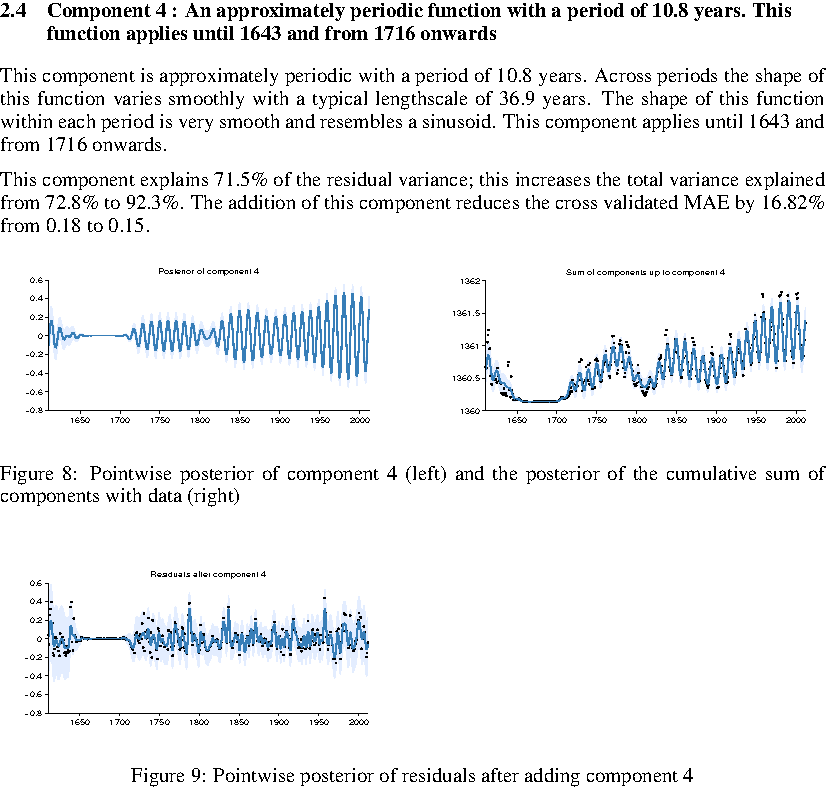
\includegraphics[trim=0cm 4.75cm 0cm 1.0cm, clip, width=0.98\columnwidth]{solarpages/pg_0007-crop}}
\caption{Extract from an automatically-generated report describing the model components discovered by automatic model search.  This part of the report isolates and describes the approximately 11-year sunspot cycle, also noting its disappearance during the 16th century, a time known as the Maunder minimum.}
\label{fig:periodic}
\end{figure}

In this paper,  we introduce a system for modelling time-series data
 containing the above ingredients which we call the Automatic
Bayesian Covariance Discovery (ABCD) system. The system defines an open-ended
language of Gaussian process models via a compositional grammar. The
space is searched greedily, using marginal likelihood and
the Bayesian Information Criterion (BIC) to evaluate models. The 
compositional structure of the language allows us to develop a method
for automatically translating components of the model into
natural-language descriptions of patterns in the data.

We show examples of automatically generated reports which highlight
interpretable features discovered in a variety of data sets (e.g.\
figure~\ref{fig:periodic}).  The supplementary material to this paper
includes 13 complete reports automatically generated by ABCD.

Of course, good statistical modelling requires not only
interpretability but predictive accuracy. We compare ABCD against
existing model construction techniques in terms of predictive
performance at extrapolation, and we find state-of-the-art performance
over the 13 time series. In the remainder of this paper we describe the
components of ABCD in detail. 

\section{A language of regression models}
\label{sec:improvements}

% what is regression
The general problem of regression consists of learning a function $f$
mapping from some input space $\mathcal{X}$ to some output space
$\mathcal{Y}$. We would like an expressive language which can
represent both simple parametric forms of $f$ such as linear, polynomial, \etc and also complex nonparametric functions
specified in terms of properties such as smoothness, periodicity, \etc~
Fortunately, Gaussian processes (\gp{}s) provide a very general
and analytically tractable way of capturing both simple and complex
functions. 



% what is a GP /  kernel
Gaussian processes are distributions over functions such that any
finite subset of function evaluations, $(f(x_1), f(x_2), \ldots
f(x_N))$, have a joint Gaussian distribution
\citep{rasmussen38gaussian}. A \gp{} is completely specified by its
mean function, $\mu(x)=\mathbb{E}(f(x))$ and kernel (or covariance) function
$\kernel(x,x') = \Cov(f(x),f(x'))$.
It is common practice to assume zero mean,
since marginalizing over an unknown mean function can be equivalently
expressed as a zero-mean \gp{} with a new kernel. The structure of the
kernel captures high-level properties of the unknown function, $f$,
which in turn determines how the model generalizes or extrapolates to
new data.  We therefore can define a language of regression models by
specifying a language of kernels.

% kernels can be composed
The elements of this language are a set of  base
kernels capturing different function properties, and a set of
composition rules which combine kernels to yield other valid kernels. 
Our base kernels are white noise ($\kWN$), constant ($\kC$), linear ($\kLin$), squared exponential ($\kSE$) and periodic ($\kPer$), which on their own encode for uncorrelated noise, constant functions, linear functions, smooth functions and periodic functions respectively.
The composition rules are addition and multiplication:
%Addition and multiplication are defined as pointwise addition and multiplication of kernel functions:
\begin{align}
k_1 + k_2 =& \,\, k_1(x,x') + k_2(x,x')\\
k_1 \times k_2 =& \,\, k_1(x,x') \times k_2(x,x')
\end{align}

\fTBD{This would be a good place to mention how kernels combine to form megatron}

% relation to previous paper
This kernel composition framework (with different base kernels) was described by \citet{DuvLloGroetal13}.
We extend and adapt this framework in several ways.
In particular, we have found that incorporating changepoints into the language is essential for
realistic models of time series (\eg figure~\ref{fig:periodic}). 
Changepoints can be defined through addition and multiplication with sigmoidal functions:
\begin{align}
\kCP(\kernel_1, \kernel_2) = \kernel_1 \times \boldsymbol\sigma + \kernel_2 \times \boldsymbol{\bar\sigma}
\label{eq:cp}
\end{align}
where $\boldsymbol\sigma(x,x') = \sigma(x)\sigma(x')$ and $\boldsymbol{\bar\sigma}(x,x') = (1-\sigma(x))(1-\sigma(x'))$.
%Changewindows $\kCW(\cdot,\cdot)$ can be defined similarly by replacing $\sigma(x)$ with a product of two sigmoids.

We also reparametrised some of the base kernels so that they were more amenable to automatic description and to extend the number of common regression models included in the language.
Table~\ref{table:motifs} lists common regression models that can be expressed by our language.
%Also, by introducing the white noise kernel the language includes heteroscedastic models when multiplied by linear kernels or sigmoids.
%Moreover, in order
%to achieve the goal of producing an interpretable decomposition of the
%function, we reparameterised some kerenls.
%For example, the periodic kernel in \citep{DuvLloGroetal13} has a constant component that can be removed to improve interpretability, and the RQ kernel used by Duvenaud can be expressed as a sum of SE kernels.

\begin{table}[ht]
\centering
\begin{tabular}{l|l}
Motif & Example kernel \\
\midrule
\gp{} smoothing & $\kSE$ \\
Linear regression & $\kC + \kLin$ \\
Multiple kernel learning & $\sum \kSE$ \\
Trend, cyclical, irregular & $\sum \kSE + \sum \kPer$ \\
Fourier decomposition & $\kC + \sum \cos$ \\
Sparse spectrum \gp{}s & $\sum \cos$ \\
Spectral kernels & $\sum \SE \times \cos$ \\
Changepoints & \eg $\kCP(\kSE, \kSE)$ \\
Heteroscedasticity & \eg $\kSE + \kLin \times \kWN$
\end{tabular}
\caption{
Syntax of common regression motifs expressible in our language.
}
\label{table:motifs}
\end{table}

\section{Model Search and Evaluation}

As in \citet{DuvLloGroetal13} we explore the language of regression models using a greedy breadth-first search.
We use the same search operators, but also include additional operators to incorporate changepoints; a complete list is contained in the supplementary material. 

After each model is proposed its kernel parameters are optimised by conjugate gradient descent.
We evaluate each optimized model, $M$, using the Bayesian Information Criterion (BIC) \citep{schwarz1978estimating}:
\begin{equation}
\textrm{BIC}(M) = -2 \log p(D\given M) + p \log n
\end{equation}
where $p$ is the number of kernel parameters, $\log p(D|M)$ is the marginal likelihood of the data, $D$, and $n$ is the number of data points.
BIC trades off model fit and complexity and implements what is known as ``Bayesian Occam's Razor'' \citep[e.g.][]{rasmussen2001occam,mackay2003information}.


\section{Automatic description of regression models}
\label{sec:description}

\paragraph{Overview}

In this section, we describe how \procedurename generates natural-language descriptions of the models found by the search procedure.
There are two main features of our language of \gp{} models that allow description to be performed automatically.

First, the sometimes complicated kernel expressions found can be simplified into a sum of products.
Because a sum of kernels corresponds to a sum of functions, each product can be described separately.

Second, each kernel in a product modifies the resulting model in a consistent way.
Therefore, we can choose one kernel to be a noun, with all others being adjectives.



\paragraph{Sum of products normal form} 

First, we convert each kernel expression into a standard, simplified form.
We do this by first distributing all products of sums into a sum of products.
Next, we apply several simplifications to the kernel expression:
The product of two $\kSE$ kernels is another $\kSE$ with different parameters. Multiplying $\kWN$ by any stationary kernel ($\kC$, $\kWN$, $\kSE$, or $\kPer$) gives another $\kWN$ kernel. Multiplying any kernel by $\kC$ only changes the parameters of the original kernel.

After applying these rules, the kernel can as be written as a sum of terms of the form:
\begin{align}
K \prod_m \kLin^{(m)} \prod_n \boldsymbol\sigma^{(n)},
\label{eq:sop}
\end{align}
where $K$ is one of \kWN, \kC, \kSE, $\prod_k \kPer^{(k)}$ or $\kSE \prod_k \kPer^{(k)}$
where $\kLin^m$ denotes a product of $m$ $\kLin$ kernels, possibly with different parameters.


\paragraph{Sums of kernels are sums of functions}
Formally, if $f_1(x) \dist \gp{}(0, \kernel_1)$ and independently $f_2(x) \dist \gp{}(0, \kernel_2)$ then ${f_1(x) + f_2(x) \dist \gp{}(0, \kernel_1 + \kernel_2)}$.
This lets us describe each product of kernels separately.


\paragraph{Each kernel in a product modifies a model in a consistent way}
This property allows us to describe the contribution of each kernel in a product with a different adjective.

Next, we describe how each type of kernel modifies a model and the corresponding description.

\begin{itemize}
\item {\bf Multiplication by $\kSE$} removes long range correlations from a model since $\kSE(x,x')$ decreases monotonically to 0 as $|x - x'|$ increases.
This can be described as making an existing model's correlation structure `local' or `approximate'.
\item {\bf Multiplication by $\kLin$} is equivalent to multiplying the function being modeled by a linear function.
If $f(x) \dist \gp{}(0, \kernel)$, then $xf(x) \dist \gp{}\left(0, k \times \kLin \right)$.
This causes the standard deviation of the model to vary linearly without affecting the correlation and can be described as \eg `with linearly increasing standard deviation'.
\item {\bf Multiplication by $\boldsymbol\sigma$} is equivalent to multiplying the function being modeled by a sigmoid which means that the function goes to zero before or after some point.
This can be described as \eg `from [time]' or `until [time]'.
\item {\bf Multiplication by $\kPer$}
%leaves correlation only between points approximately one period apart.
%Therefore, multiplying by periodic can be described by simply adding 'periodic' to a description.
%When more than one periodic function is present,
modifies the correlation structure in the same way as multiplying the function by an indepedent periodic functions.
Formally, if ${f_1(x) \dist \gp{}(0, \kernel_1)}$ and ${f_2(x) \dist \gp{}(0, \kernel_2)}$ then
\begin{align}
{\textrm{Cov} \left[f_1(x)f_2(x), f_1(x')f_2(x') \right] = k_1(x,x')k_2(x,x')}.
\end{align}
This can be loosely described as \eg `modulated by a periodic function with a period of [period] [units]'.
\end{itemize}

\paragraph{Constructing a complete sentence}
To produce a complete description, we choose one kernel to be a noun which is modified by the other kernels in the product.
That is, we construct noun phrases of the form:
\begin{align*}
\textnormal{Determiner}	+	\textnormal{Premodifiers} +	\textnormal{Noun}	+	\textnormal{Postmodifiers}
\end{align*}

As an example, a kernel of the form $\kSE \times \kPer \times  \kLin \times \boldsymbol{\sigma}$ could be described as an
\begin{align*}
\underbrace{\kSE}_{\textnormal{\scriptsize approximately}} \times 
\underbrace{\kPer}_{\textnormal{\scriptsize periodic function}} \times 
\underbrace{\kLin}_{\textnormal{\scriptsize with linearly growing amplitude}} \times 
\underbrace{\boldsymbol{\sigma}}_{\textnormal{\scriptsize until 1700.}}
\end{align*}
where $\kPer$ has been selected as the head noun.

In principle, any assignment of kernels in a product to these different phrasal roles is possible, but in practice we found certain assignments to produce more interpretable phrases than others.
The head noun is chosen according to the following ordering:
\begin{align*}
\kPer > \kWN, \kSE, \kC > \prod_m \kLin^{(m)} > \prod_n \boldsymbol\sigma^{(n)}
\end{align*}
\ie $\kPer$ is always chosen as the head noun when present.
The description for the head noun is based on the type of function that the kernel encodes for when by itself. 



\subsection{Worked example}

Suppose we start with a kernel of the form
\begin{align*}
\kSE \times (\kWN \times \kLin + \kCP(\kC, \kPer)).
\end{align*}
This is converted to a sum of products:
\begin{align*}
\kSE \times \kWN \times \kLin + \kSE \times \kC \times \boldsymbol{\sigma} + \kSE \times \kPer \times \boldsymbol{\bar\sigma}.
\end{align*}
which is simplified to
\begin{align*}
\kWN \times \kLin + \kSE \times \boldsymbol{\sigma} + \kSE \times \kPer \times \boldsymbol{\bar\sigma}.
\end{align*}
%where $\emptyset$ represents the zero function.
%We use this notation in section~\ref{sec:solar}.

To descibe the first component, the head noun description for $\kWN$, `uncorrelated noise', is concatenated with a modifier for $\kLin$, `with linearly increasing standard deviation'.
%
The second component is described as `A smooth function with a lengthscale of [lengthscale] [units]', corresponding to the $\kSE$, 'which applies until [changepoint]', which corresponds to the $\boldsymbol{\sigma}$.
%
Finally, the third component is described as `An approximately periodic function with a period of [period] [units] which applies from [changepoint]'.

\fTBD{JL: We should also mention that the detailed descriptions are less modular - but not necessarily so}
\fTBD{JL: Talk about different templates based on parameters}

\section{Example descriptions of time series}
\label{sec:examples}
We demonstrate the ability of our procedure to describe a variety of patterns on two time series.
Full reports for 13 data sets are provided as supplementary material.

\subsection{Summarizing 400 Years of Solar Activity}
\label{sec:solar}

\begin{figure}[h]
\centering
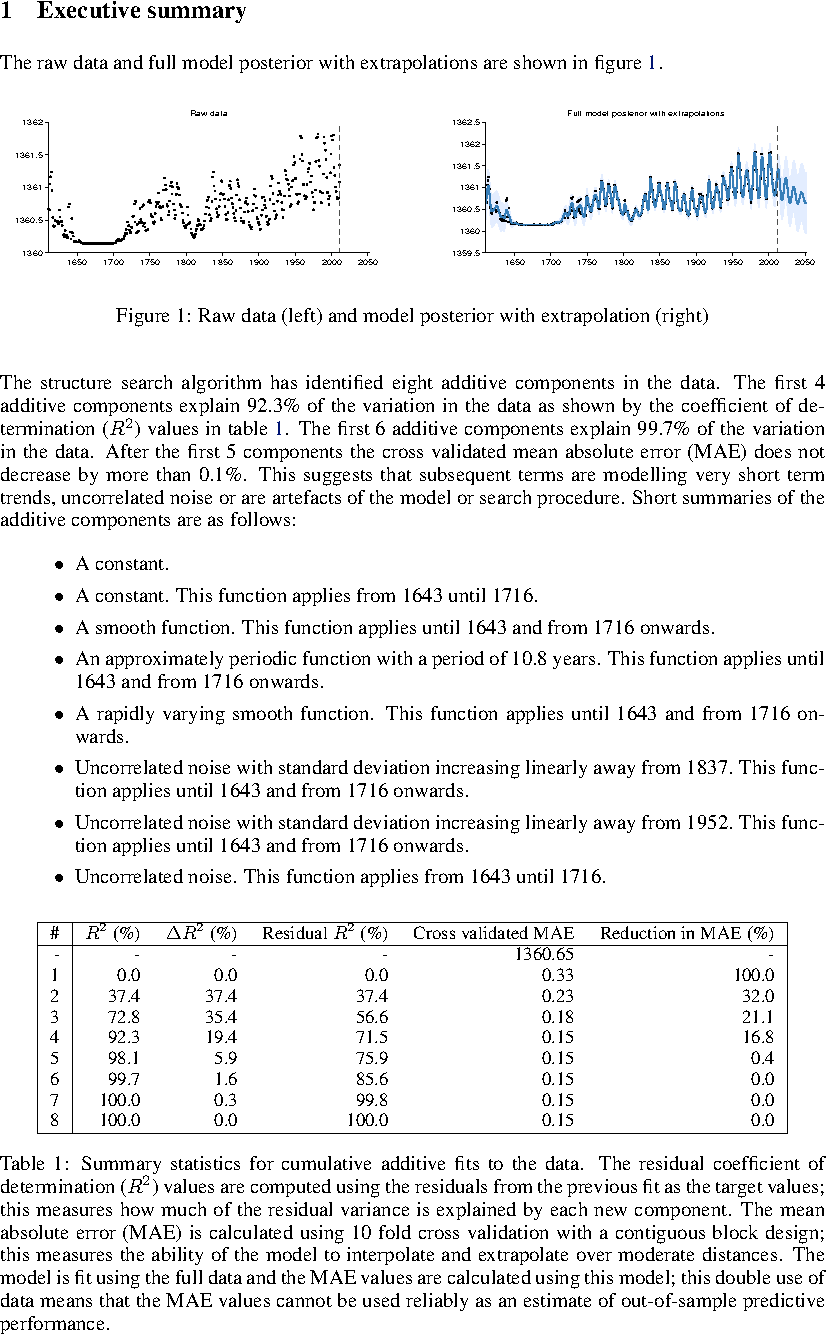
\includegraphics[trim=0.2cm 18.0cm 8cm 2cm, clip, width=0.98\columnwidth, height=0.45\columnwidth]{solarpages/pg_0002-crop}
\caption{
Solar irradiance data.}
\label{fig:solar}
\end{figure}

Here we show excerpts from the report automatically generated on annual solar irradiation data from 1610 to 2011 (figure~\ref{fig:solar}).
This time series has two pertinent features: a roughly 11-year cycle of solar activity, and a period lasting from 1645 to 1715 with much smaller variance than the rest of the dataset.
This flat region corresponds to the Maunder minimum, a period in which sunspots were extremely rare \citep{lean1995reconstruction}.
The \procedurename{} search procedure\fTBD{JL: Should we mention the search procedure - or just say that \procedurename{} has clearly identified?} and automatic description clearly identify these two features, as discussed below.

%After distributing and simplifying, the kernel corresponding to the first four components is as follows:
%\vspace{-0.5\baselineskip}
%\begin{itemize}
%  \itemsep0em
%  \item $\kC$
%  \item $\kCW(\emptyset,\kC)$
%  \item $\kCW(\kSE,\emptyset)$
%  \item $\kCW(\kSE \times \kPer,\emptyset).$
%\end{itemize}
%\vspace{-\baselineskip}
%$\kC + \kCW(\emptyset,\kC) + \kCW(\kSE,\emptyset) + \kCW(\kSE \times \kPer,\emptyset).$


\begin{figure}[h]
\centering
\fbox{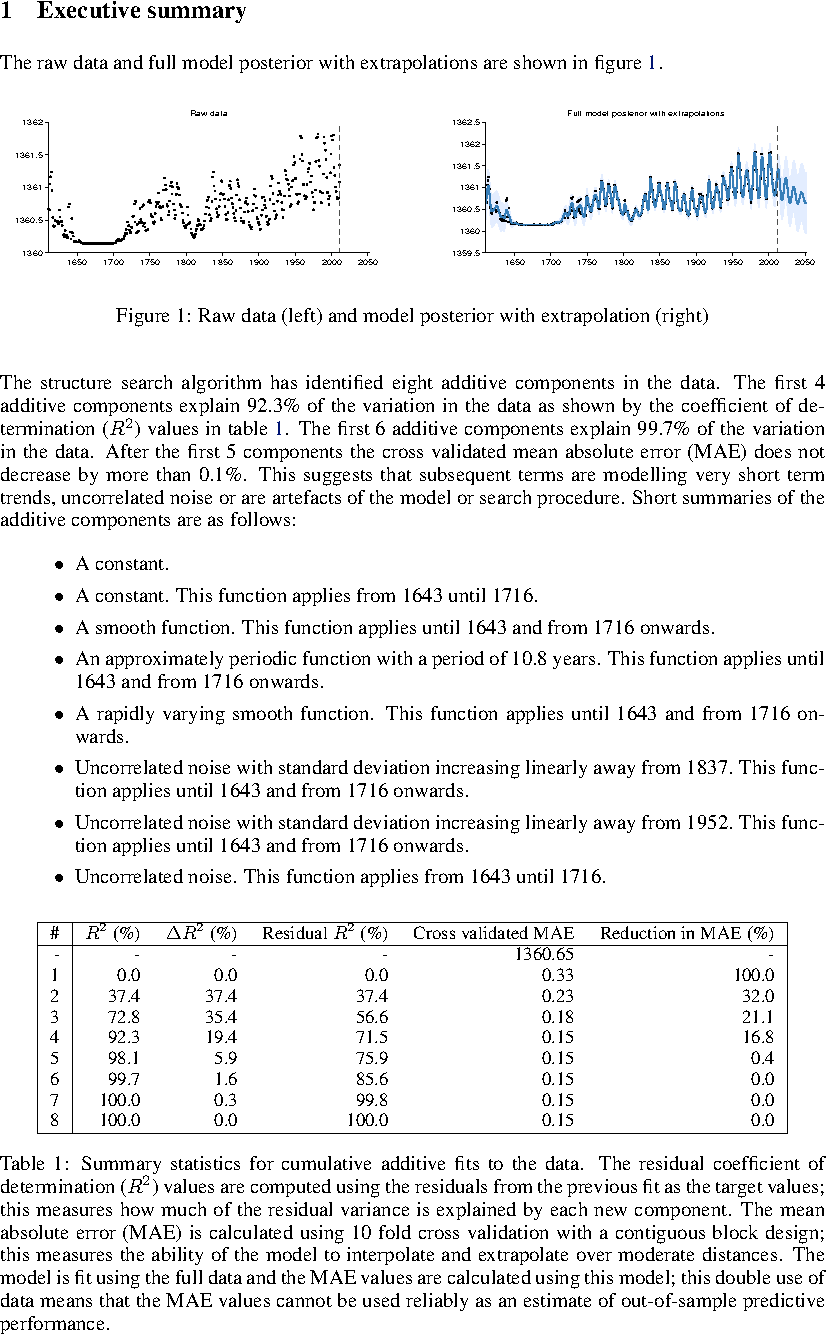
\includegraphics[trim=0cm 10.8cm 0cm 6.3cm, clip, width=0.98\columnwidth]{solarpages/pg_0002-crop}}
\caption{
An example of an automatically-generated summary of a dataset.  The dataset is decomposed into diverse structures with simple descriptions.}
\label{fig:exec}
\end{figure}
Figure \ref{fig:exec} shows the natural-language summaries of the top four components chosen by \procedurename{}.
%The short descriptions demonstrate how the kernel is split into univariate enveloping functions (from the change windows) and stationary kernels.
%
%
%The model uses 9 additive components to explain the data, and reports that the first 4 components explain more than 90\% of the variance in the data.
%This might seem incongruous with the observation that there are two main features of the data, but if we examine the first four components, we see that the first component is describing the mean of the dataset, the second is the Maunder minimum, the third describes the long-term trend, and the fourth describes the 11-year periodicity.
From these short summaries, we can see that our system has identified the Maunder minimum (second component) and 11-year solar cycle (fourth component).
These components are visualized in figures~\ref{fig:maunder} and \ref{fig:periodic}, respectively. 
By examining the parameters of the kernels representing the solar cycle, \procedurename{} identified that the shape of the periodicity is near sinusoidal and also quantifies how quickly the exact shape of the sinusoid changes.
The third component corresponds to long-term trends, as visualized in figure~\ref{fig:smooth}.
%Next, we discuss each component in greater detail.
%This might seem incongruous with the observation that there are two main features of the data, but if we examine the first four components, we see that the first component is describing the mean of the dataset, the second is the Maunder minimum, the third describes the long-term trend, and the fourth describes the 11-year periodicity.

%\subsubsection{Signal versus Noise}
%
%One design challenge we encountered was seperating the recovered structure into signal and noise.  Originally, the model always included a term corresponding to \iid{} additive Gaussian noise.  However, in practice, the distinction between signal and noise is unclear for two reasons.  First, a component which varies arbitrarily quickly in time can be indistinguishable from noise.  Second, the variance of the noise may change over time (called heteroscedasticity), and this sort of pattern may be considered part of the signal.
%Because of the blurry distinction between signal and noise, we include a table which summarizes the relative contribution of each component in terms of held-out predictive power.%  To do this, we order the components in terms of how much each one improves predictive performance in a 10-fold cross-validation procedure.  The intuition for this metric is that noise-like components do not contribute much to the extrapolation performance of the model, but that signal-like components do.
%
%
%\begin{figure}
%\centering
%\fbox{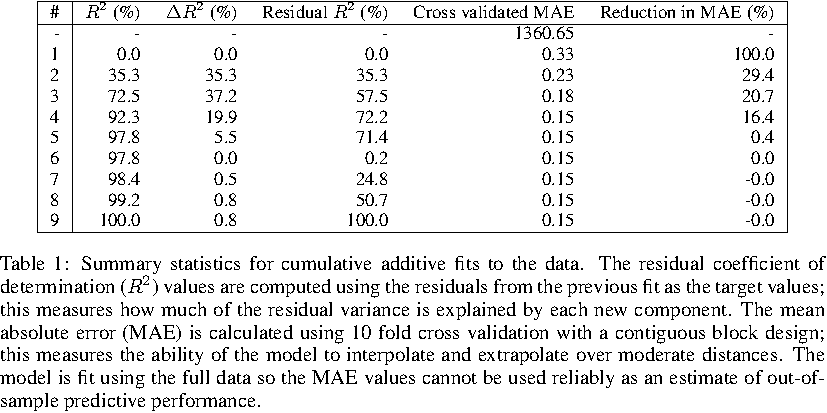
\includegraphics[width=0.98\columnwidth]{solarpages/02-solar-seperate-pages-3}}
%\caption{A table summarizing the relative contribution of the 9 different components of the model in terms of predictive performance.}
%\label{fig:table}
%\end{figure}
%
%Figure \ref{fig:table} show an example of this table on the solar dataset.

%Because the user may be interested in local or noisy components, we report all components to the user.  
%An interactive version of our procedure could allow users to specify which components are of interest, and group the remaining components into a single noise component.

%\paragraph{Decomposition plots}

%The second section of each report contains a detailed discussion of each component.
%Every component is plotted, and properties of the covariance structure are described.
%Some components are not meaningful when plotted on their own, so we also include plots of the cumulative sum of components.
%\paragraph{Automatic Plotting}
%The posterior of the individual component and sum of all components so far is visualised by plots of the posterior mean and variance.
%First, the posterior mean and variance of each component is plotted on its own.
%Second, the posterior mean and variance of all components shown so far is plotted against the data.
%This progression of plots 
%By contrasting each of these plots with plots of earlier components, we can see 
%shows qualitatively how each component contributes to an overall explanation of the data.
%A second paragraph explains the improvement in predictive performance gained by including this component in the model. This is the same informatino as included in the executive summary.
%\paragraph{Maunder minimum}
%Figure \ref{fig:maunder} shows that \procedurename{} has captured the unusual period of decreased solar activity from about 1645 to 1715, and is able to report this in natural language.
%
\begin{figure}[ht]
\centering
\fbox{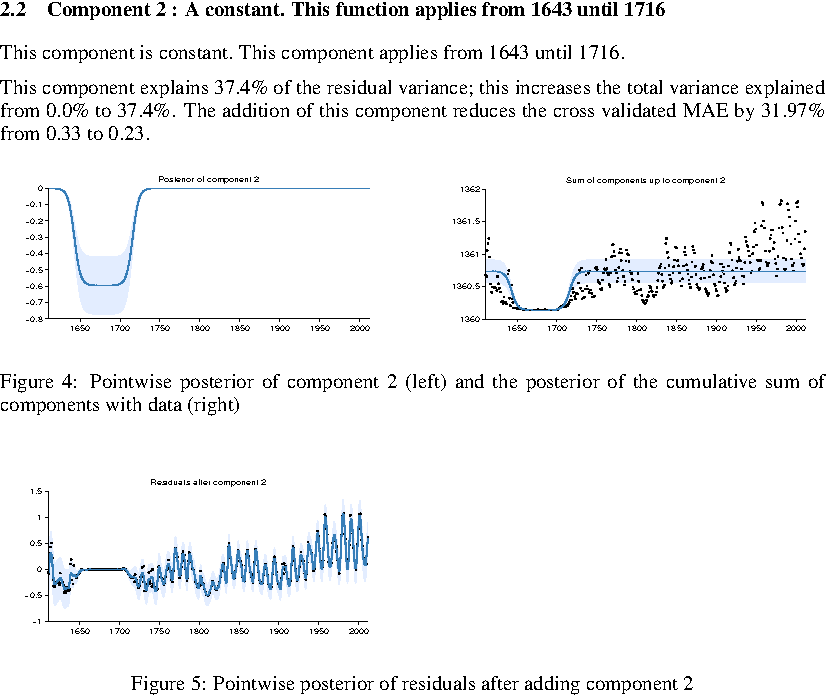
\includegraphics[trim=0cm 4.75cm 0cm 0.7cm, clip, width=0.98\columnwidth]{solarpages/pg_0005-crop}}
\caption{One of the learned components corresponds to the Maunder minimum.}
\label{fig:maunder}
\end{figure}
%
%\paragraph{Long term trend}
%
%Having isolated the Maunder minimum, the model captures the long-term trend of the rest of the data, shown in figure~\ref{fig:smooth}.
%
\begin{figure}[h!]
\centering
\fbox{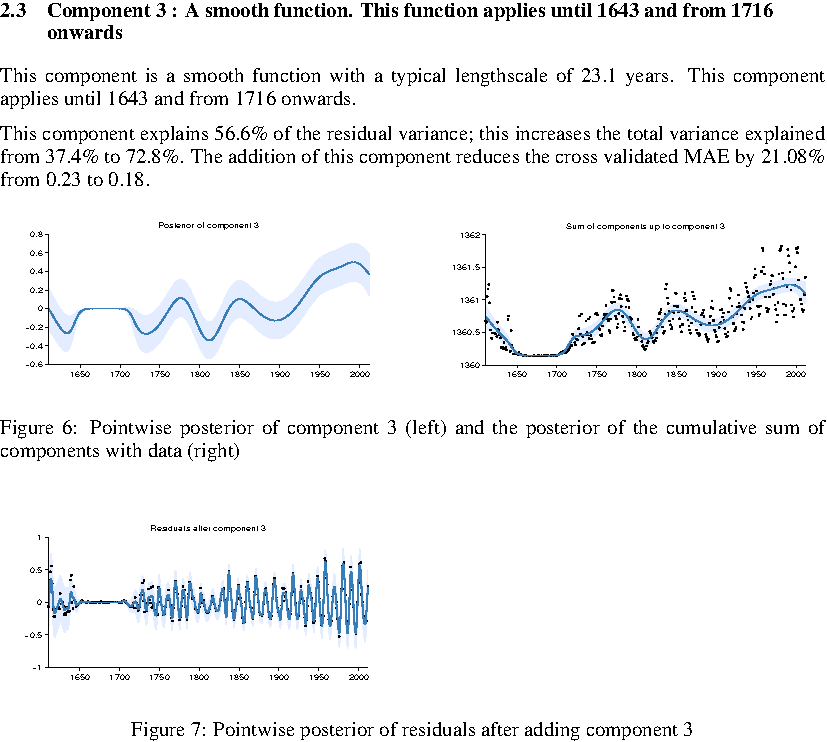
\includegraphics[trim=0cm 4.75cm 0cm 1cm, clip, width=0.98\columnwidth]{solarpages/pg_0006-crop}}
\caption{Characterizing the medium-term smoothness of solar activity levels.  By allowing other components to explain the periodicity, noise, and the Maunder minimum, \procedurename{} can isolate the part of the signal best explained by a slowly-varying trend.}
\label{fig:smooth}
\end{figure}
%
% is a good example of a meaningful component discovered by \procedurename, whose meaning would be unclear without an individual plot.  
%
%
%In the history of solar activity, the Maunder minimum is a good example of a local change in covariance.  Specifically, 
%The changepoint kernels used by \procedurename encode changes in covariance structure.
%For example, from about 1645 to 1715, solar activity decreased.
%, and very few sunspots were observed, a period called the Maunder Minimum \citep{lean1995reconstruction}.
%This feature was captured by the model by multiplying a constant kernel by two changepoint kernels.
%
%\paragraph{Solar cycles}
%
%Figure \ref{fig:periodic} shows that \procedurename{} has isolated the approximately 11 year solar cycle.

%
%with a pair of changepoint kernels.%shows exactly which sort of structure was recovered by this component.
%
%\begin{figure}[h!]
%\centering
%\fbox{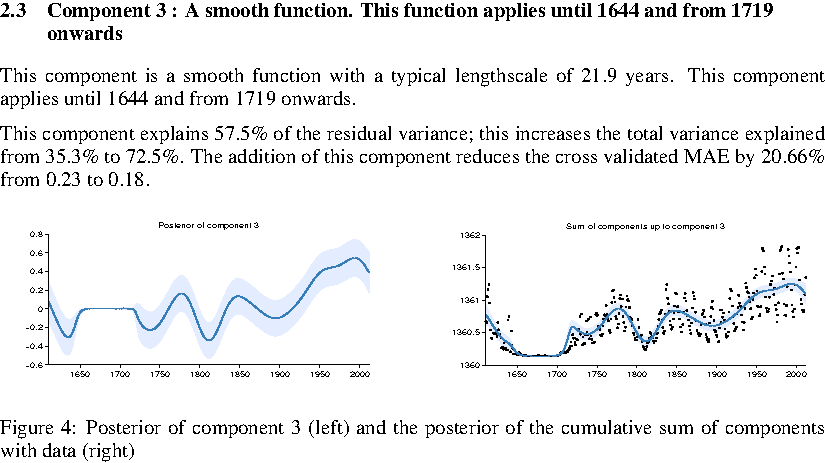
\includegraphics[width=0.98\columnwidth]{solarpages/02-solar-seperate-pages-6}}
%\caption{Characterizing the medium-term smoothness of solar activity levels.  By allowing other components to explain the periodicity, noise, and the Maunder minimum, we can isolate the part of the signal best explained by a slowly-varying trend.}
%\label{fig:smooth}
%\end{figure}
%
%\paragraph{Isolating the smoothly-varying component} Examining the dataset by eye, overall solar activity seems to change slowly over decades.  However, this intuition seems difficult to formalize.  Linear or quadratic regression is clearly inappropriate, and methods based on local smoothing would need to control for the periodic component.  Luckily, the \procedurename procedure does exactly this, allowing us to isolate the slowly-varying component of the data, without having to forecast either the Maunder minimum or the periodic variation.  Figure \ref{fig:smooth} shows the automatically-generated summary of this component.



%Figure \ref{fig:periodic} shows that \procedurename has identified the approximately 11 year solar cycle.
%By isolating this component in separate plots it is easy to see the exact nature of the solar cycle \eg how the amplitude of this periodic component varies over time.
%This demonstrates one benefit of isolating individual components: we can now see, by eye, extra structure that was not explicitly captured by the model.  Specifically, we can see that the amplitude of the periodic component varies over time.

%and by comparing with figure \ref{fig:smooth}, we can see that it varies roughly in proportion to the overall magnitude of the signal.
%  This pattern suggests that some sort of log-transform might be appropriate for this dataset, or that the model should be extended in some way to capture this structure.

%\paragraph{Extrapolation plots}
%
%The third section of each report shows extrapolations into the future, as well as posterior samples from each individual component of the model.  These samples help to characterize the uncertainty expressed by the model, and the extent to which different components contribute to predicting the future behavior of a time series.
%%
%The predictive mean and variance of the signals shown in the summary plots are useful, but do not capture the joint correlation structure in the posterior.  Showing posterior samples is a simple and universal way to illustrate joint statistical structure.
%%
%\begin{figure}[ht]
%\centering
%\fbox{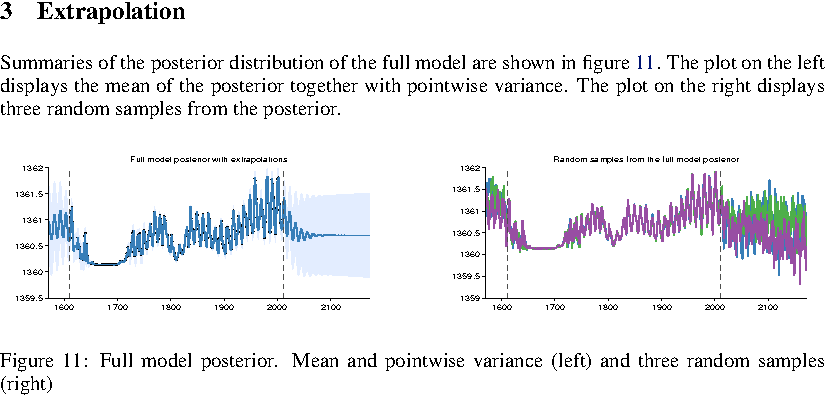
\includegraphics[trim=0cm 0cm 0cm 2.8cm, clip, width=0.98\columnwidth]{solarpages/02-solar-seperate-pages-13}}
%\caption{Sampling from the posterior.  These samples help show not just the predictive mean and variance, but also the predictive covariance structure.  Note, for example, that the predictive mean (left) does not exhibit periodicity, but the samples (right) do.}
%\label{fig:extrap-full}
%\end{figure}
%%
%For example,
%%  shows the predictive mean and variance given the entire model. 
%it is not clear from the left-hand plot in figure \ref{fig:extrap-full} whether or not the periodicity of the dataset is expected to continue into the future.  However, from the samples on the right-hand size, we can see that this is indeed the case.  

%\begin{figure}[h!]
%\centering
%\fbox{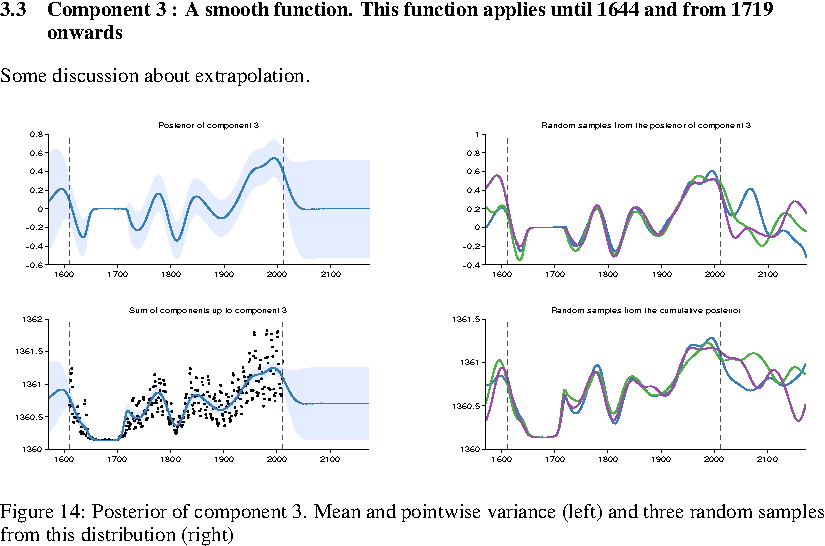
\includegraphics[width=0.98\columnwidth]{solarpages/02-solar-seperate-pages-16}}
%\caption{Extrapolating a single component of the model.  Because our model class allows us to isolate individual components, we can show the extent to which the model expects different trends to continue.  We also observe that the posterior samples are quite different from the posterior mean, away from the data.}
%\label{fig:extrap-smooth}
%\end{figure}

%\paragraph{Extrapolating individual components}
%We can also examine the model's expectations about the future behavior of individual components through sampling.  Further plots in the extrapolation section show posterior samples for each individual additive component. %For example, in figure \ref{fig:extrap-smooth}, we are shown samples of the predictive distribution of the smooth component of variation.  This plot indicates that the model considers a wide range of future average intensities to be plausible, but that it always expects those average intensities to vary smoothly.


\subsection{Describing heteroscedasticity}
\label{sec:airline}

\begin{figure}[h]
\centering
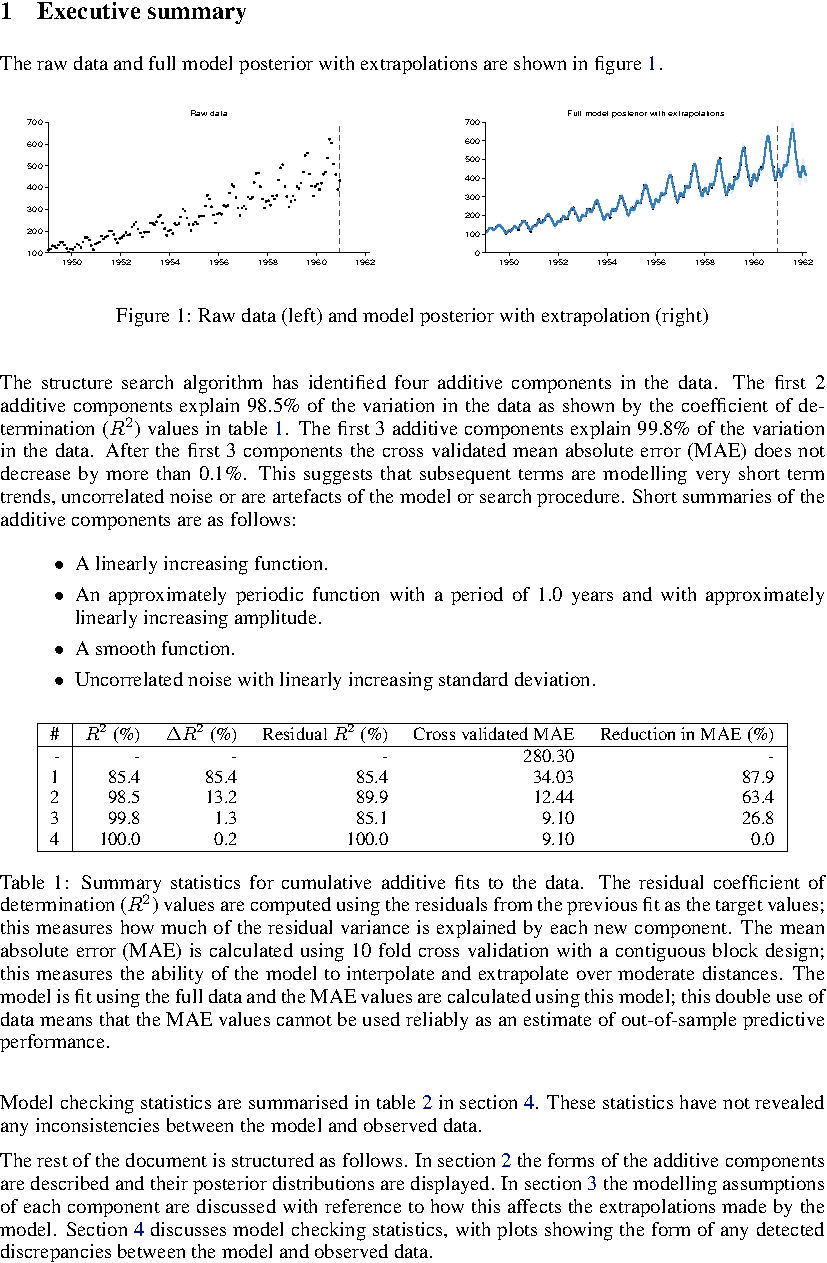
\includegraphics[trim=0.4cm 16.8cm 8cm 2cm, clip, width=0.98\columnwidth, height=0.45\columnwidth]{airlinepages/pg_0002-crop}
\caption{
International airline passenger data.}
\label{fig:airline}
\end{figure}

Next, we present the analysis generated by our procedure on international airline passenger data (figure~\ref{fig:airline}).
The model constructed by \procedurename{} has four components: $\kLin + \kSE \times \kPer \times \kLin + \kSE + \kWN \times \kLin$, with descriptions given in figure~\ref{fig:exec-airline}\fTBD{JL: The table could be cut for brevity}.
%\vspace{-0.5\baselineskip}
%\begin{itemize}
%  \itemsep0em
%  \item $\kSE$
%  \item $\kSE \times \kPer \times \kLin$
%  \item $\kSE$
%  \item $\kWN \times \kLin$
%\end{itemize}
%\vspace{-\baselineskip}
%
\begin{figure}[h]
\centering
\fbox{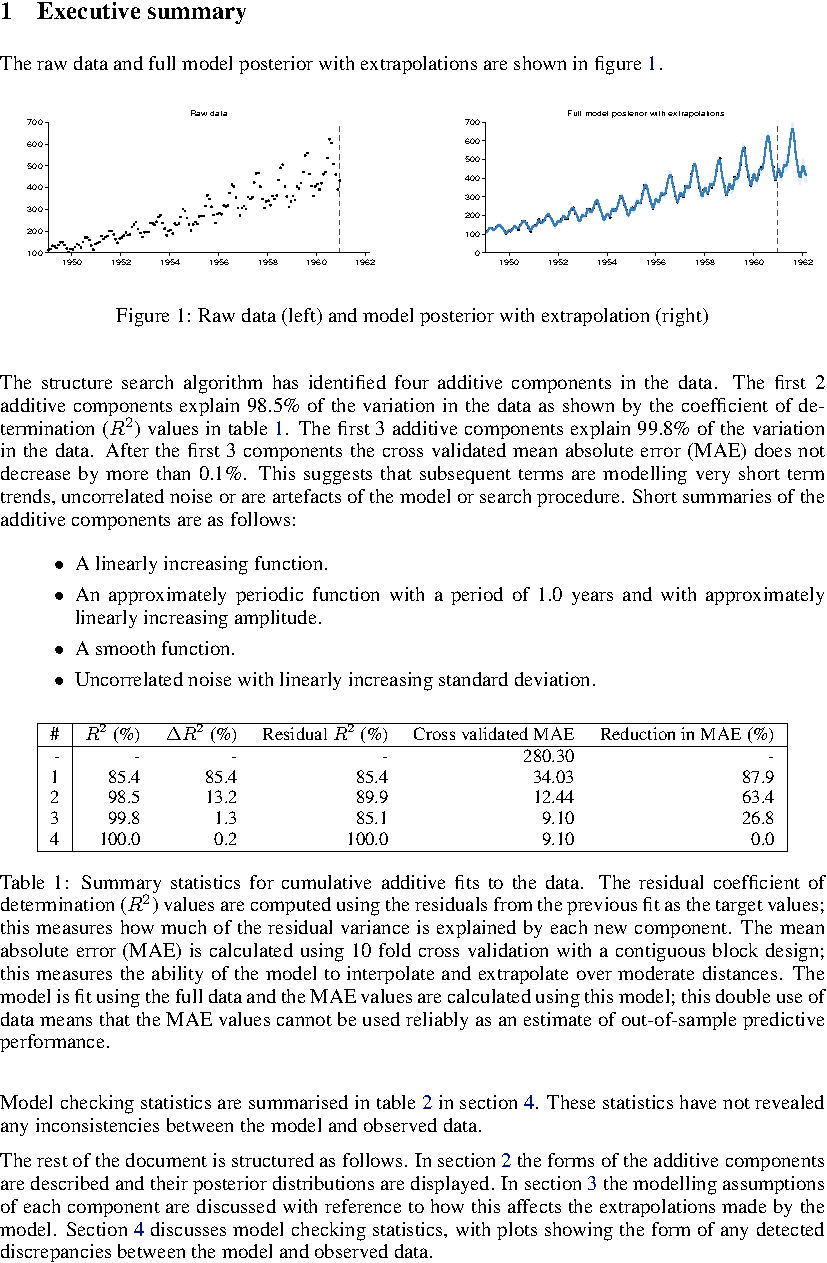
\includegraphics[trim=0cm 6.8cm 0cm 6cm, clip, width=0.98\columnwidth]{airlinepages/pg_0002-crop}}
\caption{
Short descriptions and summary statistics for the four components of the airline model.}
\label{fig:exec-airline}
\end{figure}
%
%\paragraph{Monotonic trend}
%\fTBD{JL: This will change to a linear trend in the official version - unless vetoed}
%No model in the current language can express a prior over monotonic functions.
%However, it is simple to check the posterior for monotonicity and remark upon it when appropriate (figure~\ref{fig:monotonic}).

%\begin{figure}[h]
%\centering
%\fbox{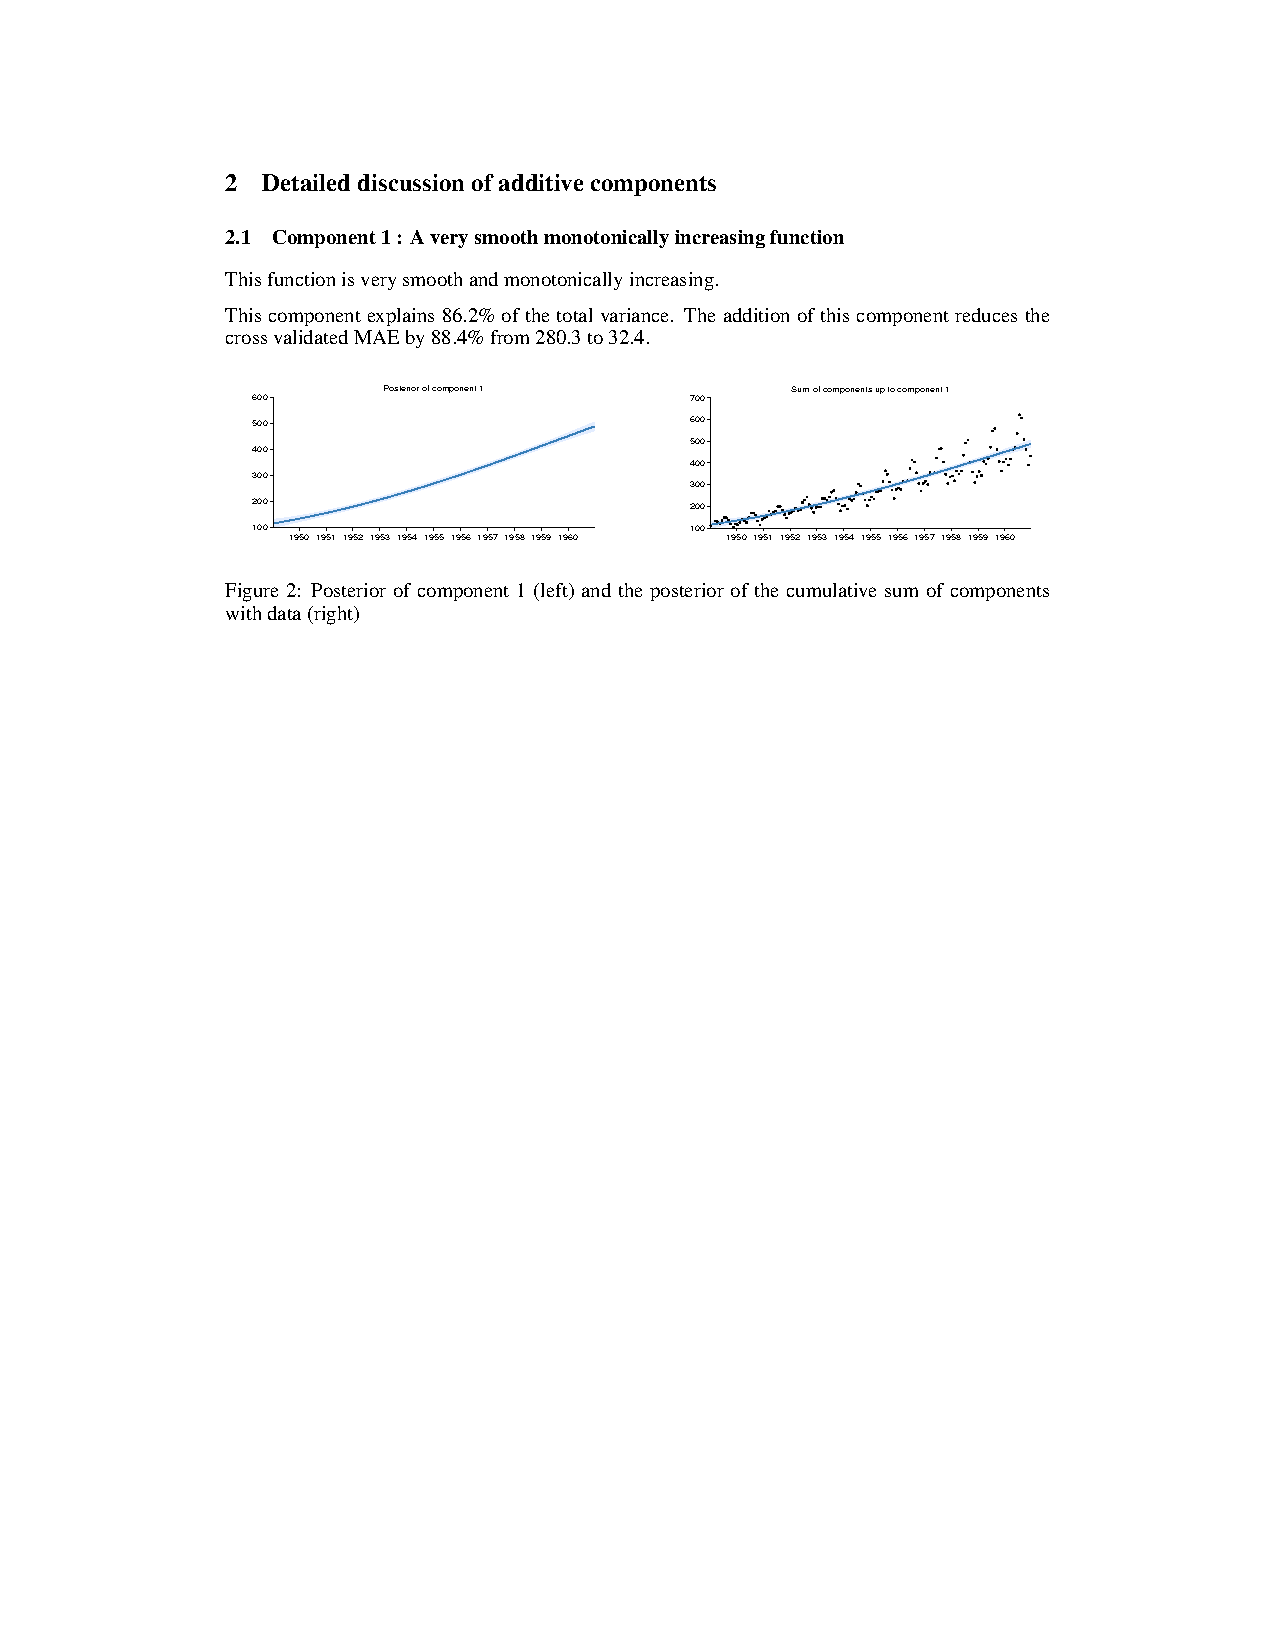
\includegraphics[trim=0cm 0cm 0cm 0cm, clip, width=0.98\columnwidth]{airlinepages/01-airline-separate-pages-3}}
%\caption{Describing monotonicity of the posterior}
%\label{fig:monotonic}
%\end{figure}

%\paragraph{Annual periodicity with linearly growing amplitude}

The second component (figure~\ref{fig:lin_periodic}) is correctly described as approximately ($\kSE$) periodic ($\kPer$) with linearly growing amplitude ($\kLin$).
%
\begin{figure}[h]
\centering
\fbox{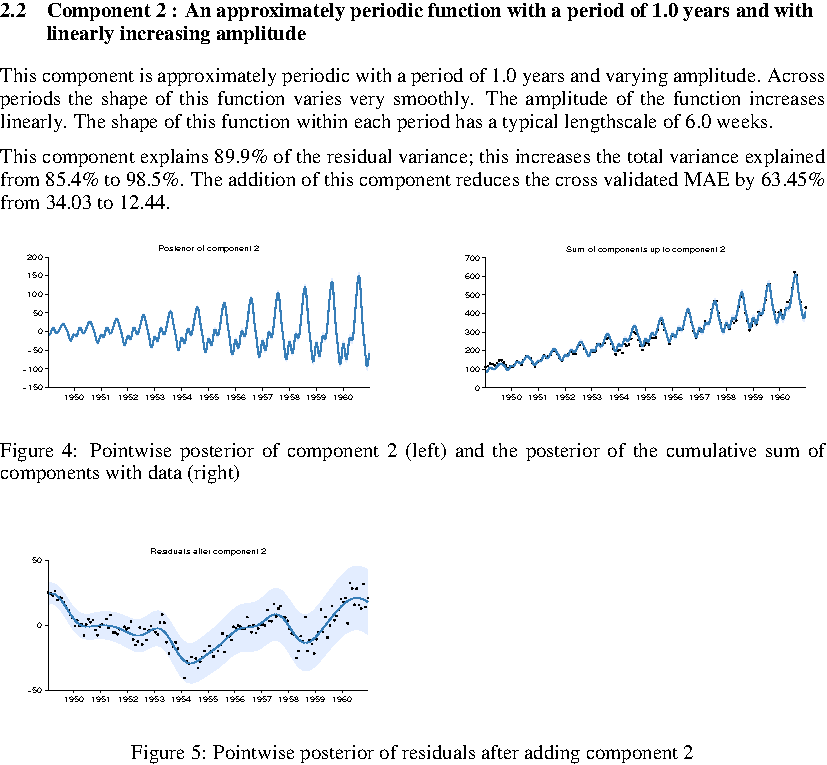
\includegraphics[trim=0cm 4.75cm 0cm 0cm, clip, width=0.98\columnwidth]{airlinepages/pg_0004-crop}}
\caption{Capturing non-stationary periodicity in the airline data}
\label{fig:lin_periodic}
\end{figure}
%
%\begin{figure}[h]
%\centering
%\fbox{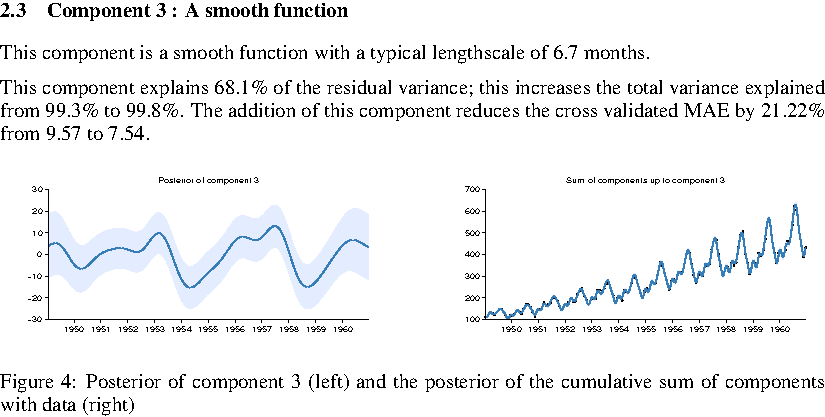
\includegraphics[trim=0cm 17cm 0cm 3.5cm, clip, width=0.98\columnwidth]{airlinepages/01-airline-separate-pages-5}}
%\caption{
%A caption.}
%\label{fig:exec}
%\end{figure}
%
%\paragraph{Linear heteroscedasticity}
%
By multiplying a white noise kernel by a linear kernel, the model is able to express heteroscedasticity (figure~\ref{fig:heteroscedastic}).
%
\begin{figure}[h]
\centering
\fbox{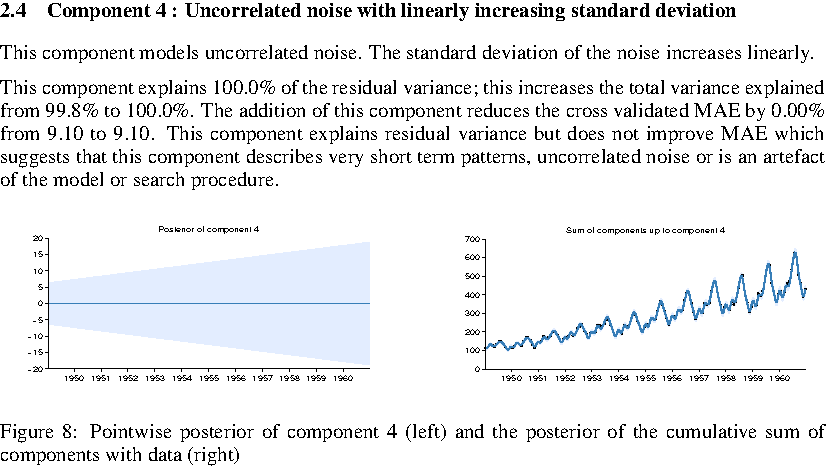
\includegraphics[trim=0cm 0cm 0cm 0cm, clip, width=0.98\columnwidth]{airlinepages/pg_0006-crop}}
\caption{Modelling heteroscedasticity}
\label{fig:heteroscedastic}
\end{figure}

\subsection{Comparison to equation learning}
\label{sec:eqn-learning-comp}

%Much of machine learning research focuses on numerical performance, with claims of interpretability generated post-hoc.
%In contrast, equation learning \citep[e.g.][]{Schmidt2009b} can also be used to automate interpretation.

Eureqa \citep{Eureqa} is a system capable of producing parametric descriptions of time-series.
Here, we show equations produced by Eureqa for the data sets shown above, using the default mean absolute error performance metric.
%\footnotetext{We experimented with the root mean squared error with Akaike information criterion penalisation (analogous to the criterion used by \procedurename{}) but occasionally observed severe overfitting.}


The learned equation for the solar irradiance data is
\begin{align*}
\textrm{Irradiance($t$)} = 1361 + \alpha\sin(\beta + \gamma t)\sin(\delta + \epsilon t^2 - \zeta t)
\end{align*}
where $t$ is time (the input to the regression) and constants are replaced with symbols for brevity.
This equation captures the constant offset of the data, and models the long term trends with a product of sinusoids, but fails to capture the solar cycle or the Maunder-minimum.

The learned equation for the airline passenger data is
\begin{align*}
\textrm{Passengers($t$)} = \alpha t + \beta\cos(\gamma - \delta t)\textrm{logistic}(\epsilon t - \zeta) - \eta
\end{align*}
which captures the approximately linear trend, and the periodic component with approximately linearly (logistic) increasing amplitude.
However, the periodicity is heavily approximated with only a single sinusoid and the model cannot capture heteroscedasticity.





\section{Related work}
\label{sec:related-work}

\paragraph{Building Structured Covariance Functions}
\cite{rasmussen38gaussian} devote 4 pages to manually constructing a complex kernel to model a time series of carbon dioxode conentrations.
In the supplementary material, we include a report automatically generated by \procedurename{} for this dataset; our procedure chose a model similar to the one they constructed by hand.
%A report automatically generated by \procedurename{} on this data set is included in the supplementary material and discovers a very similar model. 
Other examples of papers whose main contribution is to use domain knowledge to manually construct and fit a compound \gp{} kernel are \cite{klenske2012nonparametric} and \cite{lloydgefcom2012}.

\paragraph{Equation learning} \fTBD{RBG: not equation discovery?}
%In this work we have defined a search space of statistical models, where each model is characterised by a parametric covariance function.
%Previous work has considered searching over parametric functions \citep[e.g.][]{Schmidt2009b}.
%Some functions are well explained parametrically \eg a logistic function, whereas others are best described by their covariance \eg an approximately periodic function.
\cite{schmidt2009distilling}, \cite{todorovski1997declarative} and \cite{washio1999discovering} learn parametric forms of equations specifying time series, or relations between quantities.
In constrast, \procedurename{} models the covariance structure, allowing it to model functions without a simple parametric form.
%(We compare against an equation learning system in section~\ref{sec:eqn-learning-comp}.)
%Because our system specifies the more general\fTBD{JL: Sounds like we are claiming we are a super set of equation learning - we need more kernels to make this claim} covariance structure rather than the functions themselves, we are able to capture structure which does not have a simple parametric form.

\paragraph{Searching over open-ended model spaces}

This work was inspired by previous successes at searching over open-ended model spaces: matrix decompositions \citep{grosse2012exploiting}, graph structures \citep{kemp2008discovery}, and 3D scenes \cite{VikashScene13}.\fTBD{RBG: I'm not familiar with the Vikash reference; does it fit in this context?}
In all three cases, the model spaces were defined compositionally in terms of a handful of components and operators, and models were selected using criteria which trade off model complexity and closeness of fit.
Our work differs in that our procedure automatically interprets the model for the user, making the system accessible to non-experts and attenuating the biases of human interpretation.
%In another related paper, \cite{VikashScene13} automatically searches over models of 2D scenes.
%Automatic model search is possible whenever the following conditions are met: 1) we can define a large space of models by combining a small number of components in a small number of different ways; 2) inference can be performed for all models in this space; 3) a basic search procedure is sufficient to find accurate models.
%These conditions were also met for example in \citet{kemp2008discovery} who learned the structural form of a graph used to model human similarity judgments.  
%More generally, probabilistic programming [cite]\fTBD{Is there a canonical reference yet \eg I don't think there are any books} software automatically generates inference mechanisms for open-ended classes of models, enabling automatic model search.

%\fTBD{JL: Something about graphical models?}

%\NA{
%This is also true of - can we also cite some sort of graphical model work?
%}
%\fTBD{RG: Cite Kemp + Tenenbaum?}

%\paragraph{Standard inference methods}
%\fTBD{RG: How is this relevant?}
%The \procedurename language can express many regression motifs as \gp{}s for which inference is well understood.
%Probabilistic programming (cite) defines languages that describe generative models in such a way that %inference can be performed in each model.
%Extending the model search ideas in \procedurename to searches over probabilistic programs would be an interesting area for future research (cite Josh's workshop paper?).

\paragraph{Natural-language outputs}
To the best of our knowledge, our procedure is the first example of automatic description of nonparametric statistical models.
However, systems with natural language outputs have been built in the areas of video interpretation \citep{barbu2012video} and automated theorem proving \citep{GanesalingamG13}.
We agree with \citet{GanesalingamG13} that natural language outputs make it more obvious whether an algorithm's internal representations are meaningful and cognitively plausible\fTBD{JL: Strong - but I like it}.

%\section{Numerical evaluation}
\section{Predictive Accuracy}
\label{sec:numerical}

\begin{figure*}[ht]
\centering
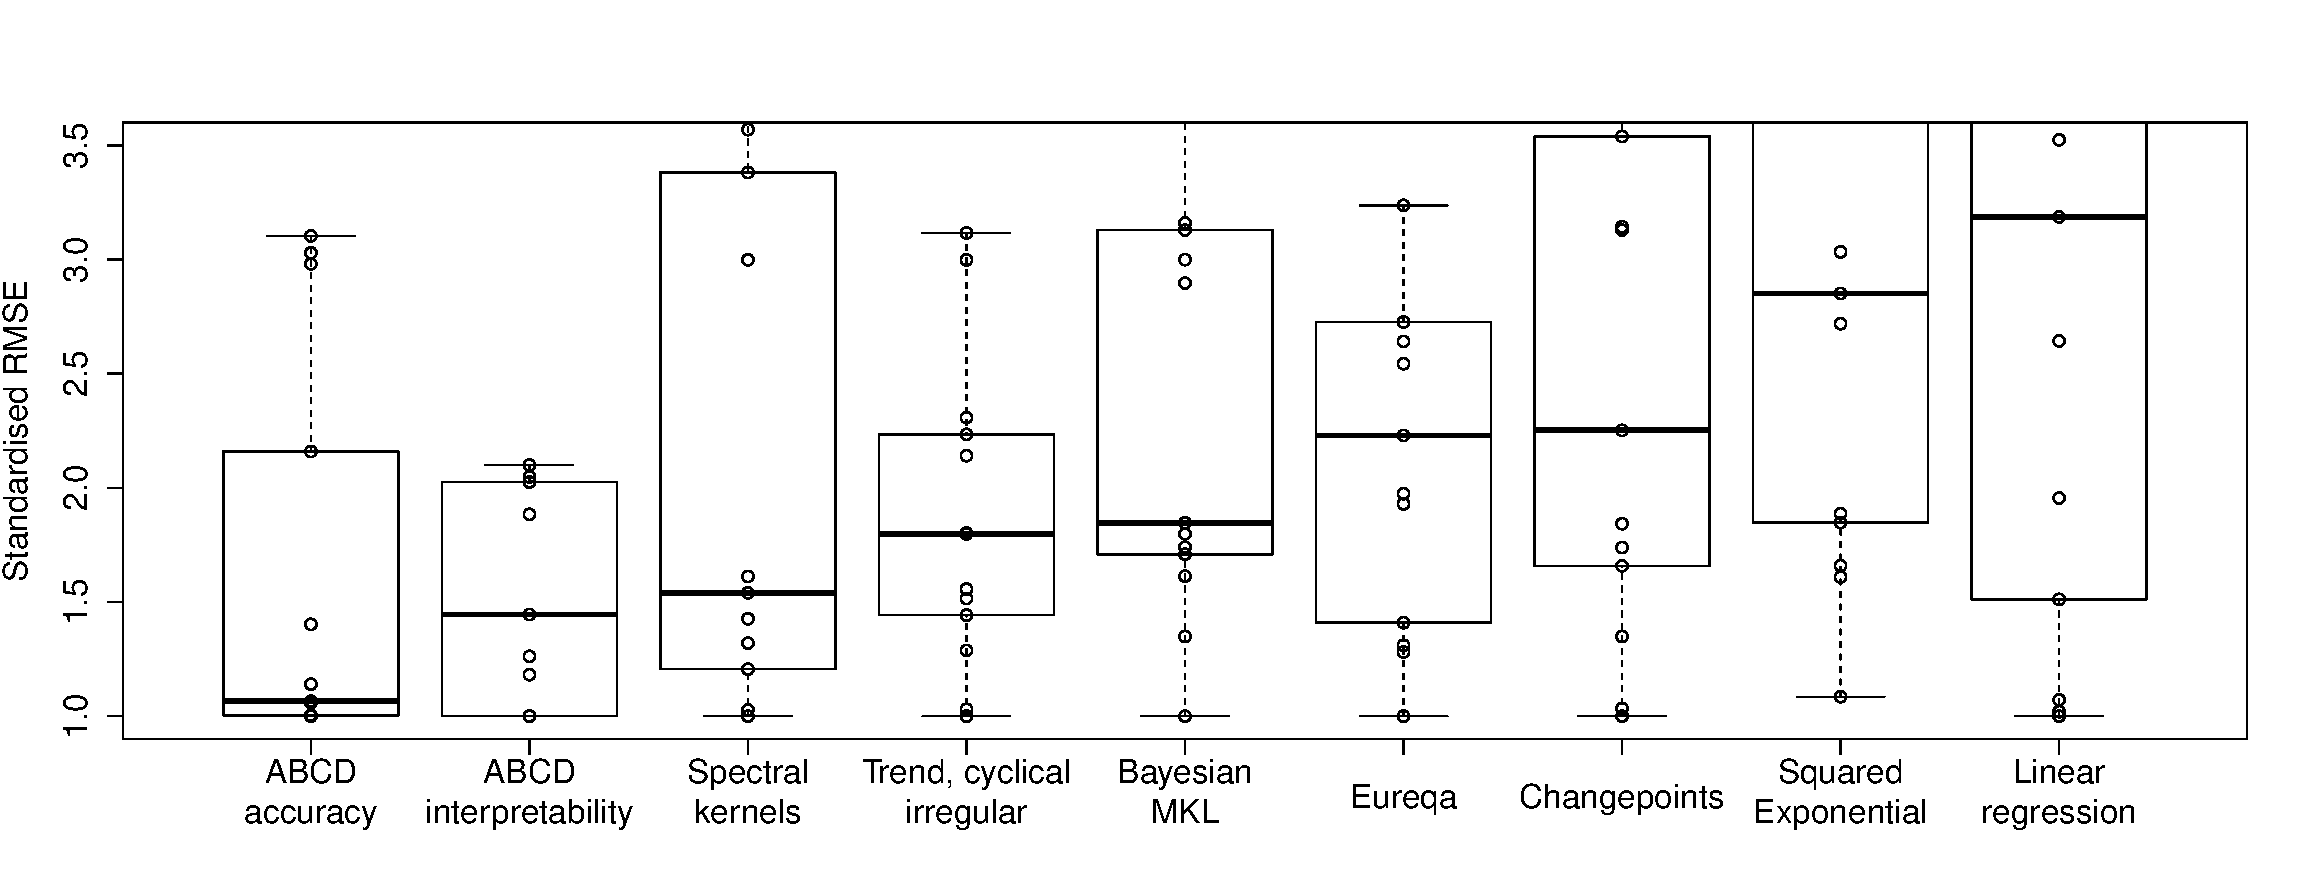
\includegraphics[width=\textwidth]{figures/box_extrap_wide}
\vspace{-0.8cm}
\caption{
Raw data, and box plot of standardised extrapolation RMSE (best performance = 1).
Ordered by median.
}
\label{fig:box_extrap_dist}
\end{figure*}

To complement our demonstration of the interpretability of \procedurename{}, we compared the predictive accuracy of various model-building algorithms at interpolating and extrapolating time-series.
On these datasets, \procedurename{} outperforms the other methods on average.% on average (\eg as measured by quantiles of performance metrics).
%\NA{However, the variability of the results suggests that there is room to improve the robustness of \procedurename.}
%\fTBD{JL: I'm trying to avoid claims of oversell - any thoughts on a measured statement?}

\paragraph{Data sets}

In addition to the three time series analysed by \cite{DuvLloGroetal13} we evaluate the performance of the algorithms listed below on 10 additional time series from the time series data library \citep{TSDL}; plots of the data can be found at the beginning of the reports in the supplementary material.

\paragraph{Algorithms}

We compare the structure search algorithm to equation learning using Eureqa \citep{Eureqa} and six other regression algorithms: linear regression, \gp{} regression with a single $\kSE$ kernel (squared exponential), a Bayesian variant of multiple kernel learning \citep{bach2004multiple}, change point modelling
% / multi resolution Gaussian processes 
\citep{garnett2010sequential, FoxDunson:NIPS2012}, spectral kernels \citep{WilAda13} and trend-cyclical-irregular \citep[e.g.][]{lind2006basic}\fTBD{Can anyone find a more academic reference?}.

We use the default mean absolute error criterion when using Eureqa.
All other algorithms can be expressed as restrictions of our modelling language (see table~\ref{table:motifs})\fTBD{JL: This link needs to be fixed or the table reintroduced EARLY} so we perform inference using the same search methodology and selection criterion\footnotemark~(Bayesian information criterion) with appropriate restrictions to the grammar.
For MKL, trend-cyclical-irregular and spectral kernels, this search corresponds to forward-selection.
\footnotetext{We experimented with using unpenalised conditional likelihood as the search criterion for other methods but observed overfitting, as is to be expected.} 

We restricted to regression algorithms for comparability; this excludes models which regress on previous values of times series \citep[e.g.][]{box2013time}.
Producing model construction algorithms for this class of time-series model would be an interesting area for future research.

\paragraph{Interpretability versus accuracy}

The search procedure sometimes produces kernel expressions having many nested products of sums, resulting in descriptions containing many relatively uninterpretable components\fTBD{JL: This is a weak sentence - maybe we should revert to the previous version}.  In order to encourage the search to report fewer, more interpretable components, we experimented with forcing the search procedure to always distribute products during search.  We call this procedure \procedurename{}-interpretability, in contrast to the unrestricted version of the search, \procedurename{}-accuracy, which tends to produce models with better predictive performance.  \procedurename{}-interpretability was used to produce the reports shown in this paper, and we compare the performance of both in the prediction experiments.
%After applying search operators to a kernel we distributed all products over addition, changepoint and changewindow operators and simplified the resulting expression.
%This variant (\procedurename{} interpretability) of the search tends to produce models with fewer additive components improving interpretability.
%We also include the unrestricted version of the search (\procedurename{} accuracy) which tends to produce models that are better at extrapolation and interpolation.
%
%The research leading up to this manuscript has focused on interpretability.
%One could almost certainly improve the numerical results presented in this section by reintroducing $\kRQ$ and including Mat\'ern kernels as well as others.
%We leave a full exploration of the interpretability / accuracy trade-off for future work.

\paragraph{Extrapolation}

To test extrapolation we trained all algorithms on the first 90\% of the data, predicted the remaining 10\% and then computed the root mean squared error (RMSE).
The RMSEs are then standardised by dividing by the smallest RMSE for each data set so that the best performance on each data set will have a value of 1.
%
Figure~\ref{fig:box_extrap_dist} shows the standardised RMSEs across algorithms.
%Both versions of \procedurename{} have lower quartiles than all other methods but the outliers of \procedurename{}, TCI and SP have similar values.

Overall, the model construction methods with the greater capacity perform better: trend-cyclical-irregular outperforms Bayesian MKL, which outperforms squared exponential.
Eureqa performs relatively poorly, since very few datasets are well explained by a parametric equation.

Not shown on the plot are large outliers for spectral kernels, Eureqa, squared exponential and linear regression with values of 11, 493, 22 and 29 respectively.
All of these outliers occurred on a data set with a large and sharp discontinuity (see the call centre data in the supplementary material).
%All methods attempted to model this discontinuity using inappropriate components resulting in wild predictions.

%Also not shown on the plot is a very large outlier for EL of 493 (this was also on the call centre data).
%However, EL was the best performing algorithm on the wages dataset which shows an exponential increase after the industrial revolution.
%\procedurename can approximate an exponential function with a polynomial by combining $\kLin$ kernels but this is not a succinct expression in the current language.
%Expanding the modelling language of \procedurename is a natural area for future research.

%Somewhat surprisingly, TCI performs well despite its restrictive modelling assumptions (smooth functions and exact periodicity).
%Further inspection of the extrapolation has revealed that while TCI cannot model non-stationarity, its extrapolations of approximately periodic components can be quite effective.
%While \procedurename and SP will quickly become uncertain about a roughly periodic component, TCI will predict the average which is often more effective.
%This suggests that models composed of kernels of the form $(\kSE + \kC) \times \kPer$ will be effective for extrapolating approximately periodic components.

\paragraph{Interpolation}
To test the ability of the methods to interpolate, we randomly divided each data set into equal amounts of training data and testing data.
%We trained each algorithm on the training half of the data, produced predictions for the remaining half and then computed standardised RMSEs.
The results are similar to those for extrapolation and are included in the supplementary material.





\section{Discussion}

We have introduced a system that can automatically find\fTBD{JL: Surely construct or build?} appropriate models from an open-ended space and generate natural language reports which highlight\fTBD{JL: Explain / describe?} underlying sources of variability.
%To the best of our knowledge this is the first system that can automatically describe any model in an open-ended class of nonparametric models in natural language.
Our procedure's extrapolation and interpolation performance are also competitive with existing model construction techniques.
This can be seen as the beginnings of an automated statistician, which would make nonparametric regression models accessible to non-experts.


%Thinking towards extending this line of work many questions and challenges are raised which we briefly outline.

%\paragraph{Accuracy versus interpretability}
% DD: we already talk about this in the experimental section
%Typical machine learning research focuses on predictive performance rather than interpretability, likely due to the difficulty of assessing the interpretability of a method in an objective manner.
%Requiring that statistical models can be automatically described constrains the models that can be used over and above the traditional constraints of tractability.

%\paragraph{A sufficiently large class of models}
%To be non-trivial.

%\paragraph{Computational complexity}
%\fTBD{JL,DD: This can potentially be shortened - or even removed}
%\fTBD{JL: At the least it should not be a verbatim quote of JBT}
%\procedurename{} is embarassingly parallel, and can be run overnight on a cluster.
%This is computationally expensive compared to fitting only one or a small number of models.
%However, this computational cost may be reasonable when compared to the cost of having a human researcher iteratively propose, fit, and refine a series of models, especially when one considers the size and scope of the space of models that is searched, and the fact that all steps of model construction, evaluation and search are automatic.

%In our experience, working statisticians, machine learners, and data scientists rarely if ever explore such a space so systematically, partly because of the cost in terms of both their own time and computation time.
%The artificial intellgience presented in this paper is still quite primitive and naive, and the space of models we can consider automatically is still quite limited compared to what humans can do.
%However, in evaluating the limitations of these methods, and prospects for future work of this sort, other factors might loom larger than computational efficiency.



%\paragraph{Automatic description of methods}



%\paragraph{When is a description of a model useful as a description of data?}

%\fTBD{Shorten me significantly}

%\procedurename produces models, $M$, of the form $f = \sum_i f_i$ where $f_i \dist \gp{}(0, \kernel_i)$.
%The form of $M$ is chosen to be that which best explains observations of $f$, denoted by $D$, as measured by approximate marginal likelihood.

%In the reports generated by \procedurename, we show plots of the posterior $p(f_i^*\given M,D)$ but the natural-language descriptions are of typical elements of the prior $p(f_i^*\given M)$ given the fitted model \ie they are descriptions of the model rather than descriptions of the data.

%Despite fitting the model to the data by maximising the marginal likelihood $p(D\given M)$ the selected model may be a poor description of the data if the data contains features not easily expressed by the language of models defined by \procedurename.
%To test for when this is the case we have begun experimenting with posterior predictive checks to assess the models produced by \procedurename following the techniques of \cite{Gelman1996} (see reports in the supplementary material).
%In fact, the posterior predictive checks take the form of comparing the expectation of statistics under the prior and posterior of each component \ie they are testing whether or not typical elements of the posterior $p(f_i^*\given M,D)$ are typical elements of $p(f_i^*\given M)$.

%However, model checking for Gaussian processes, even those with simple kernels, is under-researched so we leave their description and more detailed analysis for future work. 

%\paragraph{Other systems}
%The system presented in this paper is just one example of a system combining these elements, for performing supervised regression.
%\citep{grosse2012exploiting} provides an earlier example with builds unsupervised models.
%Similar systems could be constructed in other learning scenarios, such as sequence modeling or semi-supervised learning.

\paragraph{Source Code}
Source code to perform all experiments will be available on github upon publication.
%\href{http://www.github.com/jamesrobertlloyd/gpss-research}
%{\texttt{github.com/jamesrobertlloyd/gpss-research}}}
%All \gp{} hyperparameter tuning was performed by automated calls to the GPML toolbox\footnote{Available at 
%\href{http://www.gaussianprocess.org/gpml/code/}
%{\texttt{www.gaussianprocess.org/gpml/code/}}
%}

%\section{Discussion}

%\begin{quotation}
%``The availability of 'user-friendly' statistical software has caused authors to become increasingly careless about the logic of interpreting their results, and to rely uncritically on computer output, often using the 'default option' when something a little different (usually, but not always, a little more complicated) is correct, or at least more appropriate.''
% In trying to practice this art, the Bayesian has the advantage because his formal apparatus already developed gives him a clearer picture of what to expect, and therefore a sharper perception for recognizing the unexpected.

%\defcitealias{dyke1997avoid}{G. Dyke, 1997}
%\hspace*{\fill}\citet{Jaynes85highlyinformative}
%\hspace*{\fill}\citetalias{dyke1997avoid}
%\end{quotation}

%In this paper, we exhibited the output of a method for automatically constructing and summarizing a compositional Gaussian process regression model in natural language.
%These summaries can enable human experts and non-experts to understand the implications of a model, check its plausibility, and notice structure not yet captured by the model.

\bibliography{gpss}
\bibliographystyle{format/icml2014}

\end{document} 
